\cleardoubleemptypage
\renewcommand*\chapterpagestyle{scrheadings}
\chapter{Planning}
Planning is vital to any project, as it establishes a clear path towards success;
whilst one always needs to be creative along the way, a well-established plan
helps ensure that the final goal is clear and completable.
Setting clear goals allows the team to allocate resources properly,
which includes identifying potential risks, such as exam periods along the way
where the team does not have much time to work on the diploma thesis.
Nonetheless, remaining flexible is of utmost importance, as unexpected things
could happen in life, which may inhibit the teams ability to work for a period of time.

\section{Milestones}
Accounting for all previously mentioned points, a plan was established with clear milestones,
which would be adjusted along the way to ensure full completion was possible
and there were no periods of extended inactivity.

\begin{table}[h!]
\centering
\begin{tabular}{|l|c|}
\hline
\textbf{Milestone} & \textbf{Date} \\
\hline
Backend set up and speech recognition functions & 04.10.2024 \\
Functioning software prototype (e.g., weather querying) & 01.11.2024 \\
Components and PCB ordered & 15.11.2024 \\
Hardware and software communication functioning & 13.12.2024 \\
PCBs completed & 10.01.2025 \\
Case completed & 31.01.2025 \\
Interface with LLM & 31.01.2025 \\
Final prototype completed & 28.02.2025 \\
\hline
\end{tabular}
\caption{Project Milestones}
\end{table}

\section{System Architecture}
The project is separated into a frontend and a backend, where the frontend handles user interaction and user experience,
while the backend processes audio, turning it into a proper voice assistant output,
be that text, generated audio or an action on the system.

\subsection{Client-Server Architecture}
In the following flowchart, the frontend is depicted as the client and the backend as the server,
comunicating via a protocol that is yet to be decided depending on which ends up fitting the implementation best.

\begin{figure}[H]
\centering
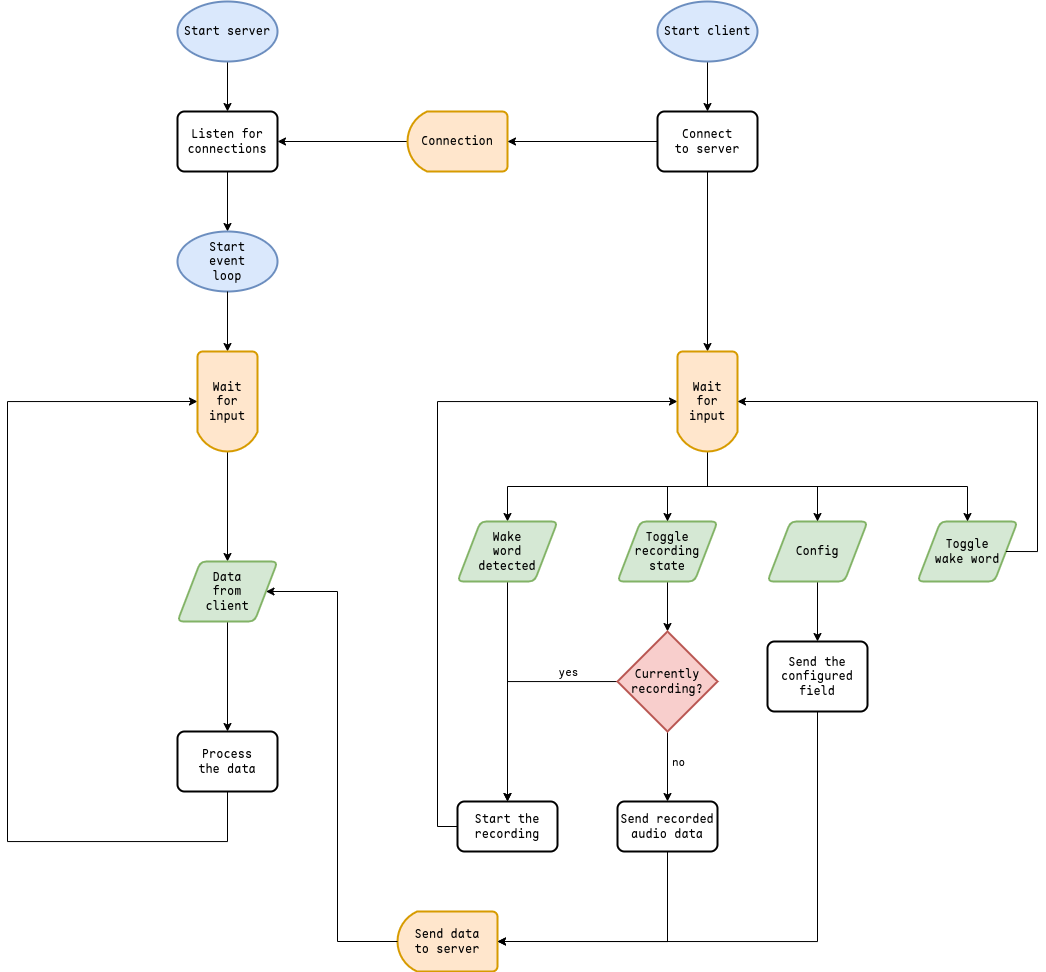
\includegraphics[width=\textwidth]{assets/architecture-pre}
\caption{Client-Server Architecture}
\label{chart:architecture-pre}
\end{figure}

The system starts with the backend listening for connections, and the client connecting to the backend.
The word connections is plural here, because the backend is intended to be able to handle multiple clients simultaneously;
having multiple configurations running at the same time would be quite a challenge to implement, and it is not planned,
especially because multiple clients would usually just mean multiple smart home nodes, which run on the same or similar hardware
and do not need varying configurations.
Once a client has connected, it should handle recording audio by itself, be that using buttons or a wake word and silence detection;
the client would send the audio to the server once finished, and the server would process it --- this is the event loop of the system.

\subsection{Configuration}
The client can send configuration commands, which will be selected from a menu on the client interface and saved into a configuration file
on the backend. TOML\footnote{Tom's obvious minimal language \cite{toml}} would be a great option because it allows for a simple table-key-value structure, allowing it to split
the configuration for different parts of the system (such as recording, transcription, or parsing) while still being able
to store key value pairs like most other configuration formats.

\subsection{Frontend}
There does not need to be a frontend for the system to function, besides for recording and playing audio; technically, all that is needed for a frontend
is an audio recorder/player and/or a text display and a client that can connect to the backend. For testing and debugging purposes, and for
the completeness of the project, a reference implementation will be created that is part of a school project and outside of the scope of this thesis.
It will be written in Qt/C++ and designed to support every feature that the backend offers, including manually recording, using a wake word and silence detection,
configuring the system, playing back audio as well as displaying text. The source code of this frontend will be hosted on GitHub\footnote{Voice Assistant reference frontend repository \cite{frontend}}.

\subsection{Language and Framework} \label{subsec:language-and-framework}
The backend will be written using Kotlin and the Spring Framework, utilizing the extensive feature set, documentation, and support the framework and the language both have.
Sprint Boot is a Java-based framework that allows developers to build huge stand-alone applications using any language that compiles to the JVM,
which are mainly Java, Kotlin, Groovy and Scala; however only Java and Kotlin are supported and maintained out of the box.
Much of its configuration is handled automatically, living by a concept called "convention over configuration"
where the user only needs to do minimal configuration to get a working application.
Out of the supported JVM languages, Kotlin was chosen for its modern approach to the JVM. It is statically typed, null safe by default,
can be both functional and object-oriented and has lots of ergonomic syntax sugar.

\subsection{Microservices}
A major issue in many large applications is the monolithic structure of the software,
where everything is tightly-coupled and changing individual bits of the program
often requires extensive and breaking changes in the event loop and other parts of the program
which should be compeletly unrelated.
This is where the microservices architecture \footnote{Microservices Architecture \cite{microservices}}
comes into play; this type of architecture organizes the program into many loosely-coupled parts
which can each have various different implementations to allow the user to choose between them.

The following flowchart shows how this structure is planned to be implemented; the event loop mentioned in the previous flowchart \ref{chart:architecture-pre}
is implemented here and can be inserted in place of the previous event loop, which only contained a brief "process the data" function.

\begin{figure}[H]
\centering
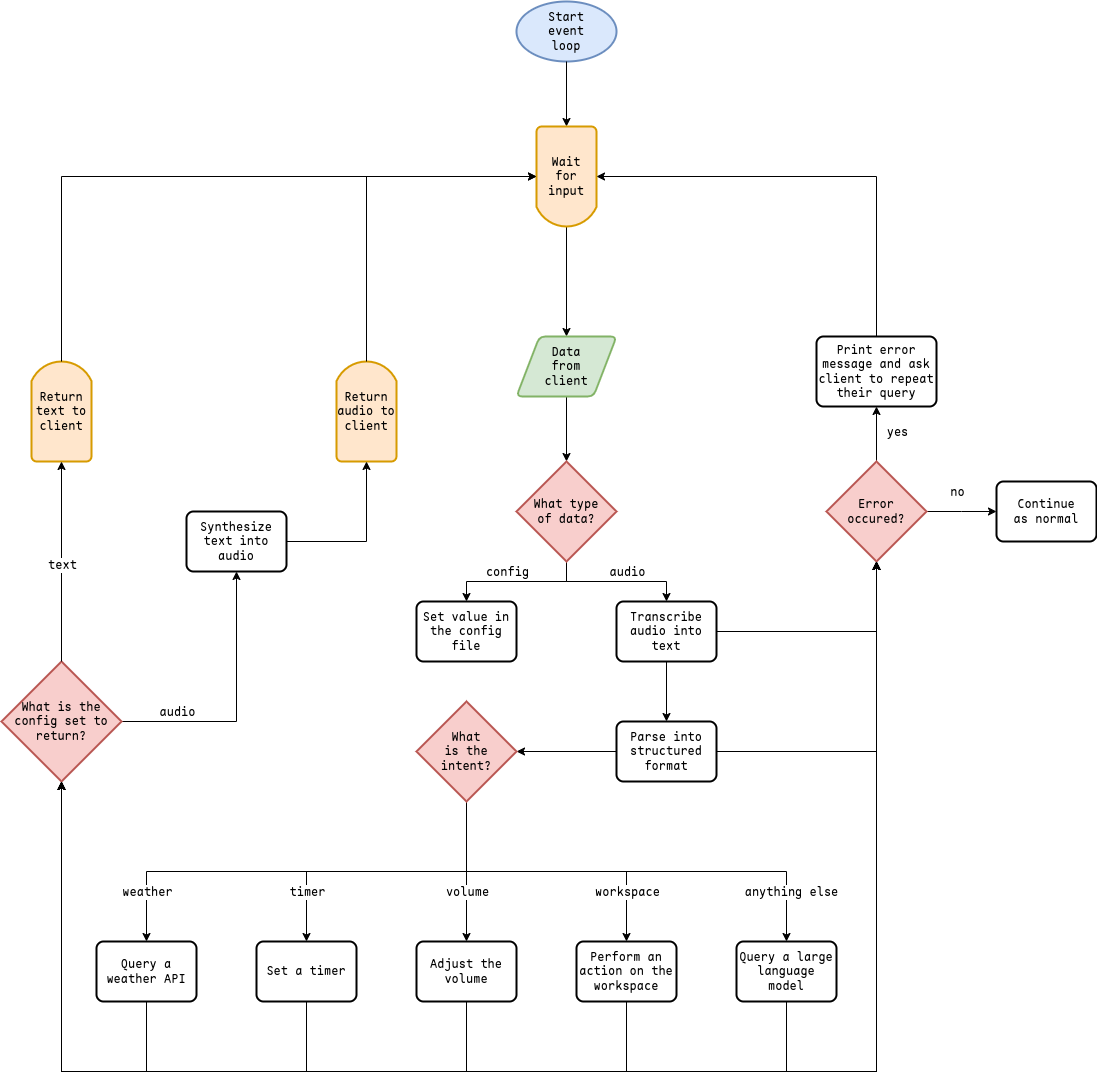
\includegraphics[width=\textwidth]{assets/processing-pre}
\caption{Client-Server Architecture}
\label{chart:processing-pre}
\end{figure}

The process starts by receiving data from the client, where this can be either audio or a configuration.
Depending on the type of data, different things are done:

If it is a configuration, then the configuration file is updated with the new value that was requested by the client.

If the data is audio, then it is processed as input; audio data is first transcribed into text using a speech-to-text microservice.
After trascription, the text is parsed using the parsing microservice, which can either be a pattern matching parser or a machine learning parser,
both of which perform natural language processing on the input text to transform it into a structured format that a computer can understand and use in the next step.
Going further, the structured format contains an intent, which, with a relatively high likelihood, is the action, which the user wants the system to perform.
The plan is to implement the most important actions which a voice assistant should have
(Querying the weather, setting a timer, moving windows on the computer, adjusting the volume, and asking an LLM), and, if there is enough time remaining, implement more actions
or allow the user to implement their own, using something akin to a YAML\footnote{YAML Ain't Markup Language\u2122 \cite{yaml}} configuration, allowing them to define
which system commands should be executed, how the voice assistant should respond or which APIs should be called when the action is performed.
After parsing everything into a simple structured action, the action will be put through a pattern matching statement, such as a switch-case or an if-else chain,
where the appropriate microservice will be invoked, depending on which intent the user most likely had.
Once the invoked microservice is done processing, its output is sent back to the client, either as text or as audio, depending on what response type the user has configured.
